\section{Notes en vrac}
\begin{itemize}
    \item Synthèse: 5 à 10 pages. Might be something good to write in english.
    \item Goal: electricity demand modeling, with forecasting for 2030. 
    \item Observer la \textbf{relation entre prix de l'électricité et changement dans la structure des moyens de production} ces dernières années $\to$ besoins de meilleures variables ?? Ou juste regarder le PIB, contrôler pour l'IPC, etc.
    \item \textbf{impact des marchés de l'électricité sur la demande d'électricité} $\to$ on juge que le prix de l'électricité capture l'effet du "marché" ??
\end{itemize}

On n'a \textit{a priori} pas d'information sur la relation analytique entre les variables : on ne suppose aucune contrainte sur les estimateurs.



\subsection{Description}
\begin{enumerate}
    \item Relation économétrique entre les variables. 
    \item Prévision de la variable dépendante.
\end{enumerate}
The given dataset is composed of 6 time series over electricity consumption, GDP, population, inflation, electricity price, climate index. The data is available from 1990 to 2021, with 32 observations. 
% We first tried to find more granular data, \textit{e.g.} quarterly one, but no source could provide electricity information over the 1990-2021 time period (the IAE has been charging for data since january 2025, Eurostat doesn't have reliable french data before 2005)\footnote{For inflation and GDP, we could have used INSEE database, \href{https://www.insee.fr/fr/statistiques/serie/001763852#Telechargement}{here} and \href{https://www.insee.fr/fr/statistiques/8196636?sommaire=8182908#consulter}{there}.}. From this situation, we already know that, dealing low-frequency data, we will not be able to include annual variability in our analysis, which could have been interesting for studying seasonal effects on electricity. We also will not be able to use moving average filter (\textit{e.g.} Hodrick-Prescott) to identify trends, economic cycles, and fluctuations in the GDP.

\subsection{Notes cours C. Doz}

\subsubsection{Univariate time series}
Stationary around a deterministic trend: $X_t = a + bt + Y_t$ where $(Y_t)_t \in Z$ is a stationary process. (Stationarity if esperance and variance does not depend on $t$).

White noise: variance is constant, no autocorrelation, mean is zero.

Wold theorem: any stationary process can be written as a linear combination of white noise. $X_t = m + \sum_{i=0}^{\infty} \psi_i \varepsilon_{t-i}$. \\


Lag operator: $LX_t = X_{t-1}$. Now, if $(X_t)_t$ is a stationary process:
\begin{itemize}
    \item $AR(p)$ process: $X_t = \mu + \sum_{i=1}^{p} \phi_i X_{t-i} + \varepsilon_t$.
    \item Best Linear Forecast of an $AR(p)$ process: $X^*_{t+1\vert t} = \mu + \sum_{i=1}^{p} \phi_i X_{t+1-i} + \varepsilon_t$.
    \item Moving average process $MA(q)$: $X_t = \mu + \varepsilon_t + \sum_{i=1}^{q} \theta_i \varepsilon_{t-i}$.
    \item $ARMA(p, q)$ process: $X_t = \mu + \sum_{i=1}^{p} \phi_i X_{t-i} + \varepsilon_t + \sum_{j=1}^{q} \theta_j \varepsilon_{t-j}$.
    \item \textbf{If $(X_t)_t$ is an $ARMA(p, q)$ process, autocorrelation should tend exponentially to 0 with increasing lags.}
    \item On these processes, the impact of a shock is transitory.
\end{itemize}

\textit{In our case, electricity consumption might not be ARMA processes, so we might not be able to forecast as such... it is to be tested. We have to test which variables can be considered stationary around a deterministic trend.}

Now, if $X_t = \mu + X_{t-1} + \varepsilon_t$ (random walk), we have: 
\begin{itemize}
    \item ARIMA: $(1 - L)^d \Phi(L)X_t = \mu + \theta(L) \varepsilon$
    \item On ARIMA process, the impact of a shock is permanent.
    \item Autocorrelation of $X_t$ don't exponentially tend to 0 with increasing lags.
    \item Identication and estimation of an $ARIMA(p,d,q)$ :
    \begin{enumerate}
    \item choice of d : visual inspection of the estimated
    autocorrelogram + unit root tests (see below).
    \item If $(X_t)_t$ appears to be non-stationary, study $(1-L)X_t$, etc...
    \item Choose the smallest $d$ such that $(1-L)^d X_t$ appears to be stationary.
    \item choice of (p,q) : compute $Y_t = (1-L)^d X_t$ and apply to $Y_t$ the procedure which has been presented for ARMA(p,q).
    Estimate an ARMA model for $Y_t$.
    \end{enumerate}
\end{itemize}

\subsubsection{Multivariate time series}
Let's consider a vector of time series $(X_t)_t$ with $X_t = (X_{1t}, X_{2t}, \ldots, X_{kt})$. We suppose that $(X_t)_t$ is a stationary process. 

Wold theorem: 
If $(X_t)_t$ is a stationary process and $(\varepsilon_t)_t$ is a white noise, then $(X_t)_t$ can be written as a linear combination of $(\varepsilon_t)_t$: $$X_t = m + \sum_{i=0}^{\infty} A_i \varepsilon_{t-i}, \quad A_0 = I, \sum_{i = 1}^\infty A_i < \infty$$ \\

VAR(p): $X_t = \mu + \sum_{i=1}^{p} \Phi_i X_{t-i} + \varepsilon_t \Leftrightarrow  \Phi(L)X_t = \mu + \varepsilon_t$. \\

\textit{It's not clear that IRC is a good variable to include in the VAR model: it does not seem to be an AR(1) process, or at least not with our granularity.}

To do an IRF: Cholesky decomposition to have an orthogonalized impulse response function.

\subsection{Notes Ferrara - Doz}
\begin{enumerate}
    \item Data analysis
    \item Model specification
    \item Parameter estimation
    \item Model validation by tests
    \item Macro use of the model for forecasting and policy analysis
\end{enumerate}

Bootstrap on residuals is valid if the residuals are white noise and the process is stationary. \\

ARDL: $Y_t = \alpha + \sum_{j=1}^m \beta_j X_{t-j} + \sum_{j=1}^m \gamma_j Y_{t-j} + \varepsilon_t$. 

\textbf{The model specification is generally carried out using
information criteria. }
\\

About Structural VAR: Structural shocks are supposed to be white noise processes and orthogonal to each others.

we could use short-run restrictions with Cholesky decomposition, but also Local Projection à la Jordà (2005) or sign (long-run) restrictions à la Uhlig (2005).

\subsection{OLS Regression}
For $n = 32$ observations, $k = 6$ variables, we use the following linear regression model:
\begin{align*}
    \boldsymbol{Y} & = \boldsymbol{X} \boldsymbol{\beta} + \boldsymbol{\varepsilon} \\
    \begin{bmatrix} 
        y_1 \\ y_2 \\ \vdots \\ y_n 
        \end{bmatrix} & = \begin{bmatrix}
        x_{11} & x_{12} & \cdots & x_{1k} \\ 
        x_{21} & x_{22} & \cdots & x_{2k} \\ 
        \vdots & \vdots & \ddots & \vdots \\ 
        x_{n1} & x_{n2} & \cdots & x_{nk} 
        \end{bmatrix} \begin{bmatrix}
        \beta_1 \\ \beta_2 \\ \vdots \\ \beta_k 
        \end{bmatrix} + \begin{bmatrix} 
        \varepsilon_1 \\ \varepsilon_2 \\ \vdots \\ \varepsilon_n \end{bmatrix}
\end{align*}

Ordinary Least Square (OLS) method is used to estimate the coefficients $\boldsymbol{\beta}$. It holds over the following hypothesis:
\begin{enumerate}
    \item More observations than explanatory variables
    \item Absence of multicollinearity $\to$ useful to check if we are using lags.
    \item Explanatory variables rely on data and the error term is random
    \item The expected value of the error term is zero
    \item Errors are not autocorrelated
    \item Errors are homoscedastic
    \item The error terms follow a normal distribution
\end{enumerate}

If the hypotheses 4, 5 and 6 are verified, the error term is white noise. 

The $R^2$ coefficient is used to evaluate the goodness of fit of the model. It measures the proportion of the variance in the dependent variable that is predictable from the independent variables. The adjusted $R^2$ is used to compare the goodness of fit of models with different numbers of variables.

Confidence interval for $\beta_j \in \{\beta_1, \beta_2, \ldots, \beta_k\}$ is given by a Student's t-distribution with $n - k - 1$ degrees of freedom. (\textit{is it useful?}). \\

Si l'hypothèse de non colinéarité n'est pas vérifiée, l'estimation du modèle est impossible (elle nécessiterait d'inverser une matrice singulière) alors que pour toutes les autres hypothèses l'estimation est possible mais donne un estimateur biaisé et/ou non efficace (à variance non minimale) mais il existe des corrections possibles. La normalité des erreurs est quant à elle non obligatoire mais permet de tirer de bonnes propriétés. 

\subsubsection{QQ plot}
The QQ-plot shows that the error terms are normally distributed.

Kolmogorov Smirnov: Various studies have found that, even in this corrected form, the test is less powerful for testing normality than the Shapiro–Wilk test or Anderson–Darling test.

The Shapiro–Wilk test is known not to work well in samples with many identical values. Jarque-Bera is bad for small samples $\rightarrow$ \textbf{Anderson-Darling} is better. 

\textbf{Student} and \textbf{Fisher} tests are used to test the significance of the coefficients: they depends on the normality of the residuals.

\subsubsection{homoscedasticity}
The Goldfeld–Quandt test is not very robust to specification errors. The \textbf{Breusch-Pagan} test is designed to detect only linear forms of heteroskedasticity. {White test} is more general and can detect a wider range of forms of heteroskedasticity, but cannot be used for small samples. \\

heteroskedasticity $\rightarrow$ weighted regression.

\subsubsection{Autocorrelation}
Durbin–Watson statistic (or Durbin's h statistic), which is only valid for nonstochastic regressors and for testing the possibility of a first-order autoregressive model (e.g. AR(1)) for the regression errors. The Breusch–Godfrey test has none of these restrictions, and is statistically more powerful than Durbin's h statistic. The Breusch–Godfrey test is considered to be more general than the \textbf{Ljung-Box} test because the latter requires the assumption of strict exogeneity, but the Breusch–Godfrey test does not. However, the \textbf{Breusch–Godfrey} test requires the assumptions of stronger forms of predeterminedness and conditional homoscedasticity.

\subsubsection{Multicollinerarity}
Commonly occurs in models with large numbers of parameters.

Use of Variance Inflation Factor (VIF) to detect multicollinearity. No clear threshold for VIF, and there is often a misunderstanding on how to deal with multicollinearity. \\

If multicollinearity is detected, the following methods can be used:
\begin{itemize}
    \item Remove one of the variables or combine them (not recommended)
    \item Use principal component analysis
    \item Use ridge regression: regularization method.
    \item Use LASSO: variable selection and regularization method.
    \item Use Elastic Net: linear combination of LASSO and ridge regression.
\end{itemize}

\subsection{Non-linear regression}
Mention the possible use of a Markov Switching process to account for IRC (up or down), or a price effect (low growth or strong growth) — use Catherine Doz's course for theoretical background.

What is shown by Lantz: Gauss-Newton method (Taylor linearization before OLS), or polynomial regression by minimising Mallows $C_p$ to know the polynomial order. 

\subsection{Forecast (see p.115)}
Boostrapping is useful when the error terms are non-normal. "L’application des méthodes de bootstrap sur les modèles de régression permet d’approximer la distribution des erreurs de prédiction par leur distribution empirique lorsque celle-ci est inconnue. Le bootstrap est ainsi particulièrement utile lorsque les
échantillons de données sont de petite taille et qu’il n’est pas possible de postuler que les erreurs ont une distribution gaussienne"

Guess for a growth rate with `predict` and add fluctuations based on the regression slope and the IRC fluctuation? \\

\begin{itemize}
    \item Estimation MCO du modèle
    \item Prévision MCO
    \item Initialisation de la boucle bootstrap
    \item Boucle bootstrap
    \item Construction de l’intervalle de prédiction bootstrap
\end{itemize}

Les mesures d’erreur quadratique moyenne et d’erreur moyenne absolue permettent de mesurer l’écart entre les prévisions et les observations lorsqu’on effectue
des prévisions sur des données rétrospectives. Les indicateurs obtenus à partir de la statistique U de Theil sont utilisés sur des prévisions rétrospectives afin d’évaluer si les erreurs de prévisions retranscrivent un effet de biais, de variance ou, de préférence, un
effet de covariance.

\subsection{À reproduire ! (p91 du poly)}
"Modèle de consommation d’électricité aux Etats-Unis expliquant le logarithme de la consommation d’électricité par habitant par le logarithme du revenu par habitant en monnaie constante et le logarithme du prix de l’électricité en monnaie constante." \\

"En effet, d’un point de vue économique, la consommation d’un bien dépend d’un effet de revenu et d’un effet de prix auxquels peuvent s’ajouter, le cas échéant, d’autres effets. Ici, on conserve la spécification la plus
simple où l’utilité d’un bien dépend d’un effet de richesse et d’un effet prix." \\

\textit{Dans notre cas, on ajoute l'effet de l'IRC et approxime les revenus par le PIB\footnote{Il existe une relation positive entre le PIB par habitant et le revenu des ménages par habitant, modulée par les politiques fiscales, la répartition des revenus, les structures économiques et la dynamique du marché du travail.
\begin{enumerate}
    \item Relation Positive:
    \begin{itemize}
        \item Un PIB/habitant élevé est généralement associé à un revenu des ménages plus élevé, car la croissance économique favorise l’emploi, les salaires et les opportunités économiques.
        \item Plus l’économie produit de biens et services, plus les revenus distribués dans l’économie sont susceptibles d’augmenter.
    \end{itemize}
    \item Différences en raison des prélèvements et transferts
    \begin{itemize}
        \item Taux d’imposition et de cotisations sociales : Un PIB élevé peut ne pas se traduire directement par un revenu élevé des ménages si les impôts sont importants.
        \item Redistribution : Des politiques de redistribution (prestations sociales, aides, etc.) peuvent influencer la relation entre les deux.
        \item Revenus des entreprises : Une partie du PIB est réinvestie par les entreprises sous forme de profits et ne se traduit pas directement en revenu des ménages.
    \end{itemize}
    \item Effets du marché du travail
    \begin{itemize}
        \item Si le taux de chômage est élevé, le PIB/habitant peut être relativement stable, mais le revenu des ménages peut être faible en raison d’un accès limité aux revenus du travail.
        \item La productivité du travail joue un rôle clé dans le lien entre le PIB et les salaires.
    \end{itemize}
    \item Effets sectoriels
    \begin{itemize}
        \item Un PIB dominé par des secteurs capitalistiques (finance, industrie lourde) peut générer un écart important entre PIB/hab et revenu/hab car les revenus du capital sont concentrés et peu redistribués aux ménages.
        \item À l’inverse, une économie fondée sur les services à forte intensité de main-d’œuvre peut avoir un lien plus direct entre PIB et revenu des ménages.
    \end{itemize}
\end{enumerate}}}.

\begin{equation}
    \ln{\frac{c_{elec}}{pop}} = \alpha + \beta_1 \ln{\frac{{PIB}}{pop}} + \beta_2 \ln{\frac{prix_{elec}}{IPC}} + \beta_3 IRC + \varepsilon
\end{equation}

\textit{Attenion: le PIB est en euros constants de 2020: on doit le convertir en euros constants de 2015.} 
$PIB_{2015} = PIB_{2020} \times \frac{IPC_{2015}}{IPC_{2020}}$.

Les coefficients $\beta_1$ et $\beta_2$ sont, respectivement, l’élasticité de la consommation
d’électricité par rapport au revenu et l’élasticité de la consommation d’électricité par rapport au prix. Ces coefficients mesurent la variation en pourcentage de la
consommation d’électricité par rapport, respectivement, à une variation en pourcentage du revenu et la variation et à une variation en pourcentage des prix. \\

On fait ensuite un test de Chow sur 2009 (crise économique ?; mais \textbf{se renseigner aussi sur la mise en place de la libéralisation des prix}\footnote{
    \begin{itemize}
        \item juillet 2007 : éligibilité de tous les consommateurs (dont les clients résidentiels) au marché concurrentiel de l’électricité.
        \item Entrée en vigueur du traité de Lisbonne le 1er décembre 2009.
        \item 7 décembre 2010 : loi NOME (Nouvelle Organisation du Marché de l’Électricité) qui vise à favoriser la concurrence sur le marché de l’électricité (\textit{e.g.} mise en place de l'accès régulé à l'électricité nucléaire historique).
\end{itemize}}).

Cusum est peu puissant (on accepte facilement l’hypothèse nulle). On peut ceci dit ajouter un test de Chow pas à pas entre 2007 et 2012. \\

Puis test de Cusum-square pour attester du structural break. On refait une régression sur 2009-2020, et on renouvelle le test de Cusum-square pour vérifier la stabilité temporelle du modèle. 

\subsection{Our results}
\begin{figure}[h]
    \centering
      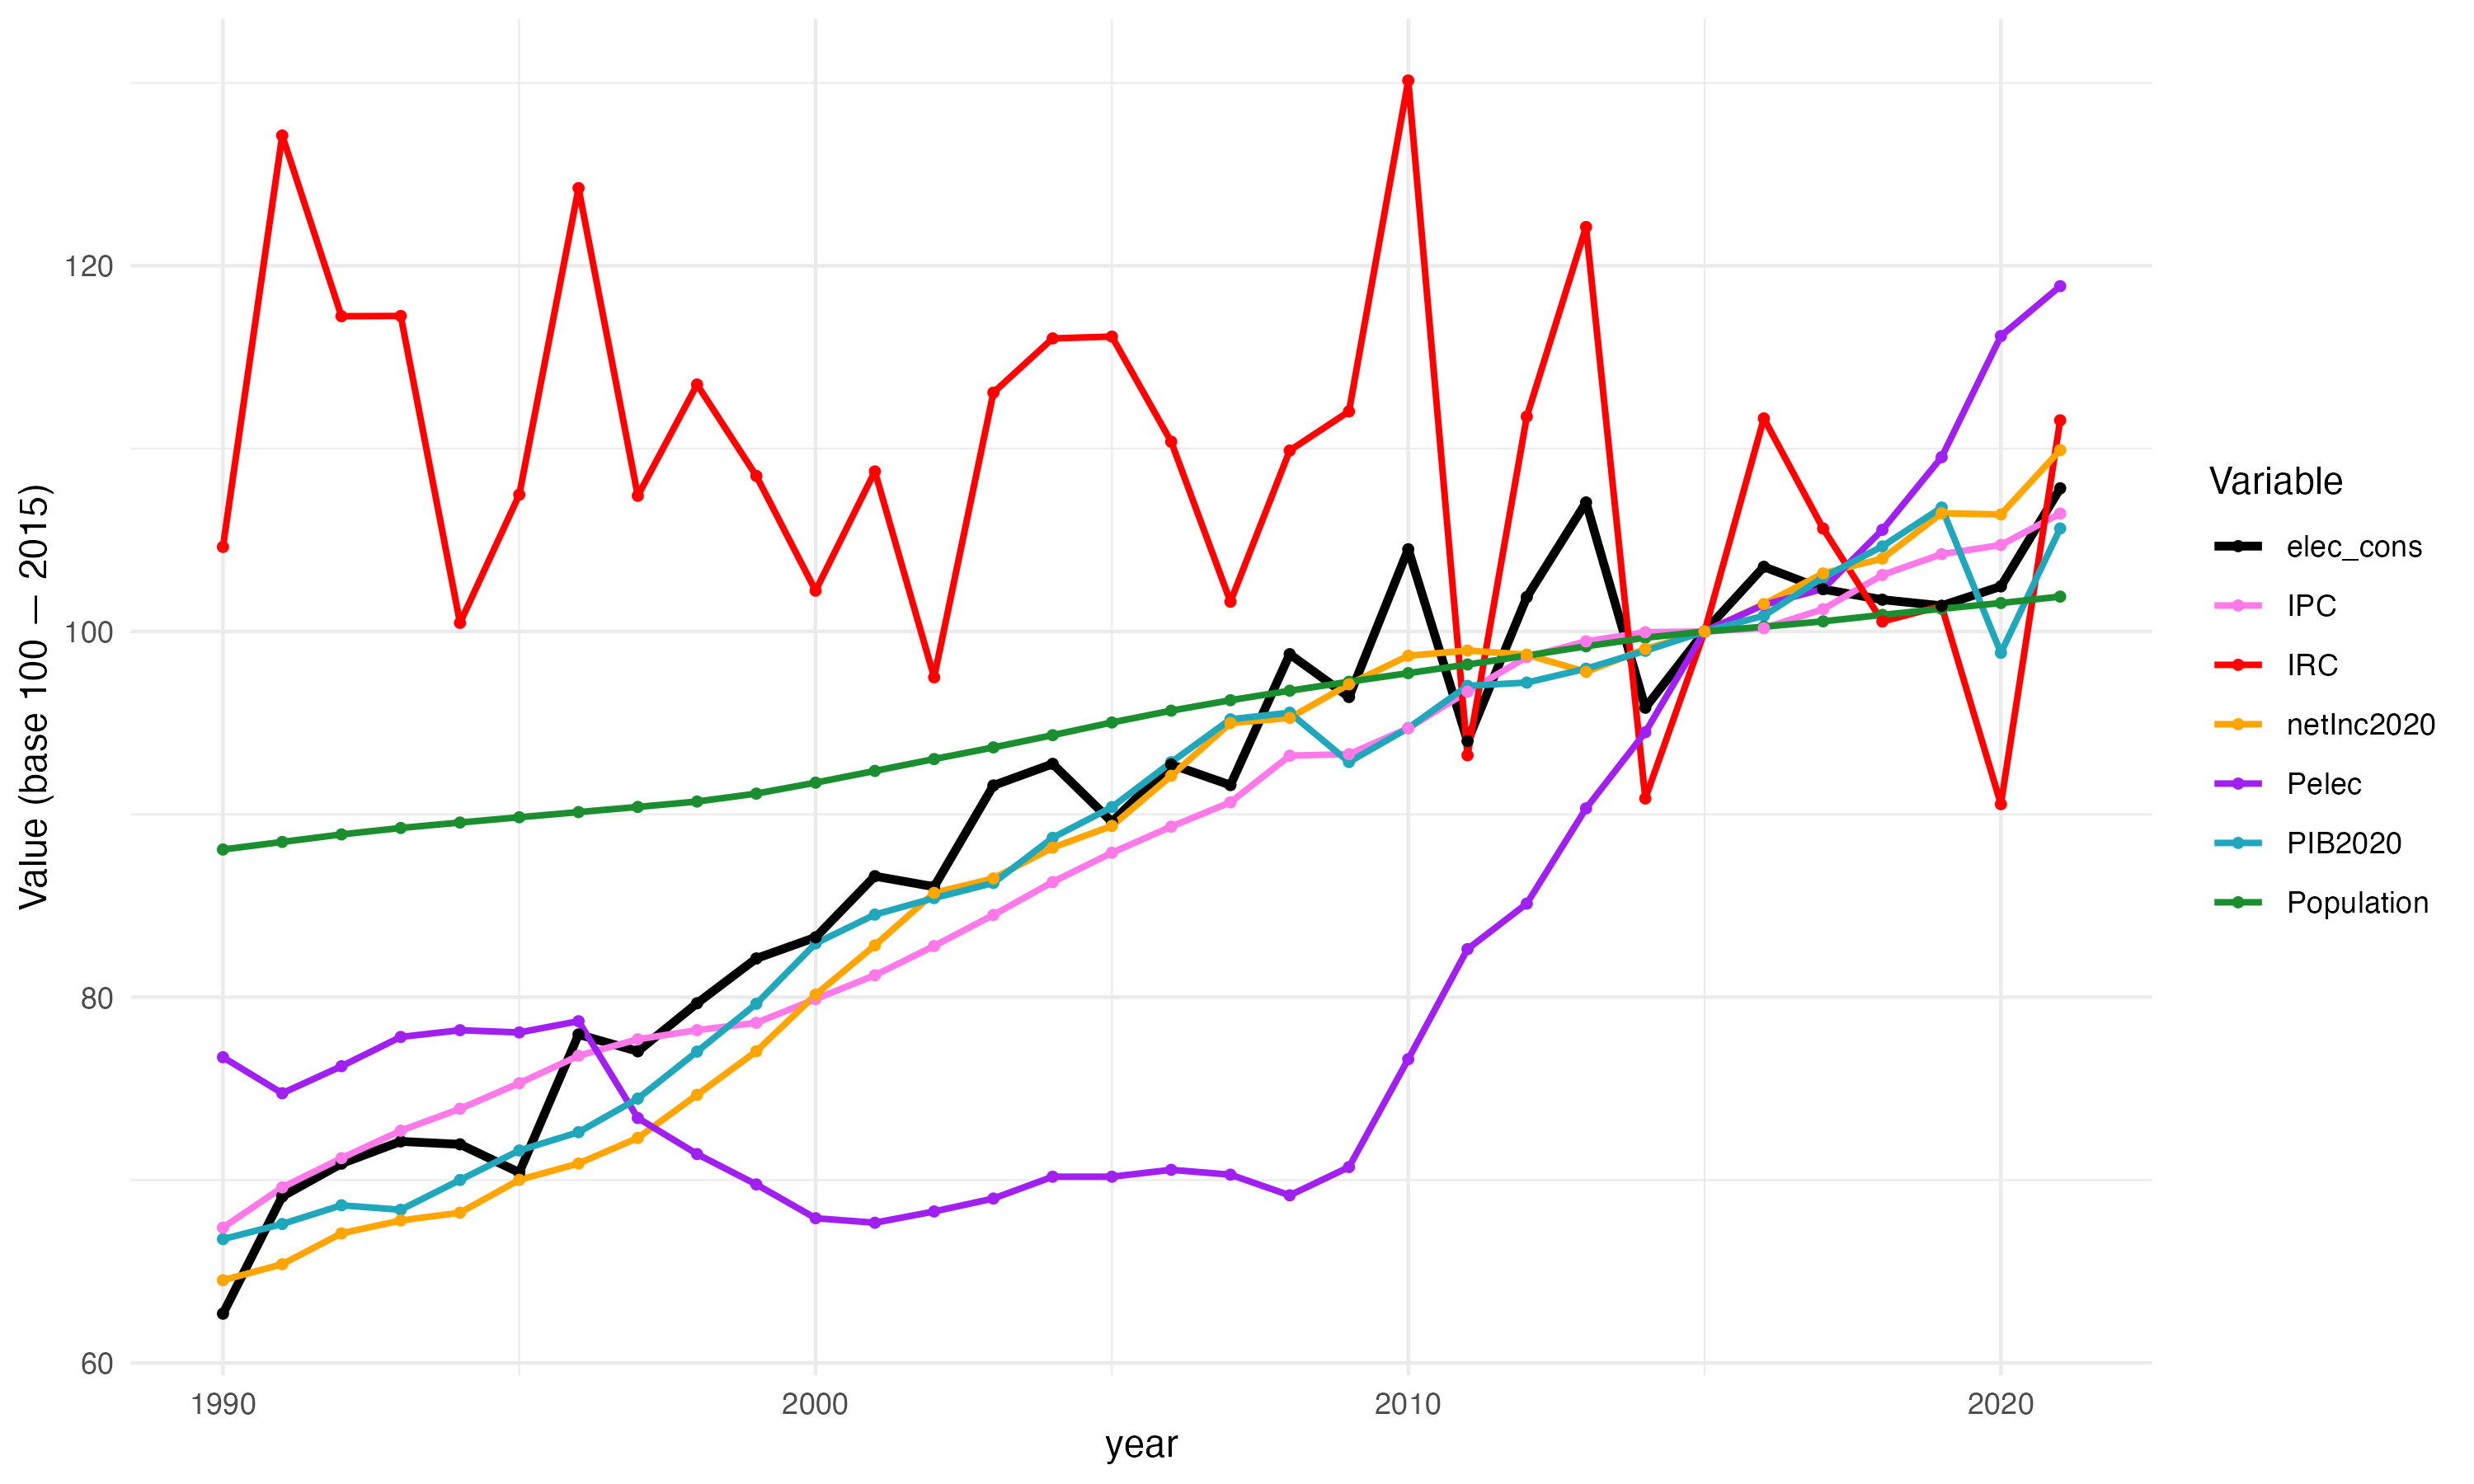
\includegraphics[width=0.54\textwidth]{Images/data_base100_2015.jpeg}
      \caption{Évolution des variables en base 100.}
          \label{var}
  \end{figure}

Graphique 1 : évolution des variables en base 100. On peut déjà intuiter une influence de la croissance du PIB, de la population et de l'indice des prix à la consommation (IPC) sur la demande d'électricité. On remarque aussi comme les fluctuations de l'Indice de Rigueur Climatique (IRC) viennent influencer la consommation d'électricité des ménages. On note enfin que la croissance forte du prix de l'électricité depuis 2009 semble corrélée à la baisse tendancielle du taux de croissance de la consommation d'électricité. Soulignons qu'à partir de cette période, le taux de croissance des prix dépasse celui de l'inflation.

\section{Introduction}
